\documentclass[12pt]{article}
\usepackage[margin=2.5cm]{geometry}
\usepackage{booktabs}
\usepackage{longtable}
\usepackage{graphicx}
\usepackage{amsmath}
\usepackage{amssymb}
\usepackage{hyperref}
\usepackage[round,authoryear]{natbib}
\usepackage{authblk}
\usepackage{array}
\usepackage{multirow}
\usepackage[utf8]{inputenc}

\title{\textbf{Supplementary Material}\\[6pt]
KNMTG: A Korean Nationwide Multimodal Transit Graph\\
for Time-Dependent Midpoint Search}
\author[1]{Yongjun Kim}
\affil[1]{Department of Software, Ajou University, Suwon 16499, Republic of Korea}
\date{}

\begin{document}
\maketitle

\section*{S1. Transfer Penalty Parameters}

Table~\ref{tab:transfer} summarises all inter-mode transfer penalties implemented
in the routing engine. Penalties were calibrated empirically to ensure that
bus-mediated shortcuts do not spuriously undercut rail boarding costs.

\begin{table}[h]
\centering
\caption{Transfer penalty values by transition type}
\label{tab:transfer}
\begin{tabular}{llr}
\toprule
From mode & To mode & Penalty (min) \\
\midrule
Any & KTX/SRT (boarding) & 20 \\
Any & GTX-A (boarding) & 8 \\
Any & Intercity bus (boarding) & 15 \\
Any & BRT (boarding) & 5 \\
Subway & Subway (same line) & 0 \\
Subway & Subway (different line) & 5 \\
KTX/SRT & Subway (at co-located station) & 10 \\
\bottomrule
\end{tabular}
\end{table}

\section*{S2. Complete Routing Test Suite}

All 33 routing test cases used for system validation are reported below
(Table~\ref{tab:tests}). Column ``KNMTG'' shows computed travel time;
``Expected'' shows the range defined in the test specification; a checkmark
indicates the result falls within the range.

\begin{longtable}{llrcp{4cm}}
\caption{Complete routing test results (33 O-D pairs)} \label{tab:tests} \\
\toprule
Origin & Destination & KNMTG (min) & Expected (min) & Note \\
\midrule
\endfirsthead
\toprule
Origin & Destination & KNMTG (min) & Expected (min) & Note \\
\midrule
\endhead
\midrule \multicolumn{5}{r}{\textit{Continued on next page}} \\
\endfoot
\bottomrule
\endlastfoot
Gangnam & Yeoksamm & 2.3 & 1--6 & Adjacent, Line 2 \\
Jongak & Sijeong & 2.7 & 1--6 & Line 1 adjacent \\
Jamsil & Jamsil-Saenae & 2.3 & 1--6 & Line 2 adjacent \\
Gangnam & Gyodae & 2.3 & 1--8 & Line 2, 2 stops \\
Gangnam & Sadang & 9.2 & 8--22 & Line 2, 7 stops \\
Jongno-3-ga & Jamsil & 34.9 & 18--40 & Line 2 + Line 5 transfer \\
Gangnam & Hongik Univ. & 39.1 & 25--45 & Line 2, 12 stops \\
Gangnam & Seoul Station & 31.4 & 25--45 & Line 2 + Line 1 transfer \\
Jamsil & Gangnam & 13.8 & 8--22 & Line 2, 7 stops \\
Gangnam & Hyehwa & 39.7 & 28--50 & 1--2 transfers \\
Gangnam & Gwanghwamun & 40.0 & 28--50 & Line 2 + Line 5 transfer \\
Gangnam & Gongdeok & 35.0 & 25--45 & Multiple paths \\
Gangnam & Jeongja & 22.5 & 18--35 & Sinbundang 5 stops direct \\
Gangnam & Pangyo & 18.0 & 14--30 & Sinbundang 4 stops direct \\
Seoul Stn. & Suwon & 22.3 & 20--80 & Saemaul direct \\
Incheon & Seoul Stn. & 72.4 & 60--95 & Line 1 end-to-end \\
Incheon & Sindorim & 56.7 & 45--80 & Line 1 \\
Incheon & Mullae & 62.5 & 50--90 & Line 1 + Line 2 \\
Incheon & Gangnam & 60.0 & 55--115 & Express bus direct \\
Yongmun & Mullae & 83.5 & 80--130 & Gyeonggi Yangpyeong \\
Yongmun & Wangsimni & 57.0 & 55--95 & Gyeongui-Jungang direct \\
Yongmun & Cheongnyangni & 39.0 & 35--90 & Gyeongui-Jungang \\
Danggogae & Sadang & 62.4 & 50--80 & Line 4 end-to-end \\
Banghwa & Hanam-Geomdansan & 100.6 & 75--115 & Line 5 Sangil branch end \\
Banghwa & Macheon & 95.7 & 70--100 & Line 5 Macheon branch end \\
Seoul KTX & Busan KTX & 141.0 & 140--200 & KTX direct \\
Seoul KTX & Dongdaegu KTX & 101.0 & 95--140 & KTX direct \\
Seoul KTX & Gwangju-Songjeong KTX & 110.0 & 100--145 & Honam KTX \\
Seoul KTX & Gangneung KTX & 106.0 & 75--130 & Gangneung KTX \\
Seoul KTX & Daejeon KTX & 56.0 & 50--85 & KTX direct \\
Gangnam & Busan KTX & 156.0 & 150--220 & Suseo (SRT) or Seoul KTX \\
Gangnam & Dongdaegu KTX & 117.9 & 110--180 & Suseo (SRT) or Seoul KTX \\
Busan KTX & Gwangju-Songjeong KTX & 162.0 & 150--280 & Via Osong transfer \\
\end{longtable}

\section*{S3. Degree Distribution Data}

The full degree distribution of KNMTG v1.1 is shown in Figure~\ref{fig:degree}.
Degree 2 (chain-like subway segments) accounts for 51.3\% of all nodes.
The long tail to degree 41 (Express Bus Terminal, Seoul) reflects the
multimodal hub function of major intercity terminals.

\begin{figure}[h]
\centering
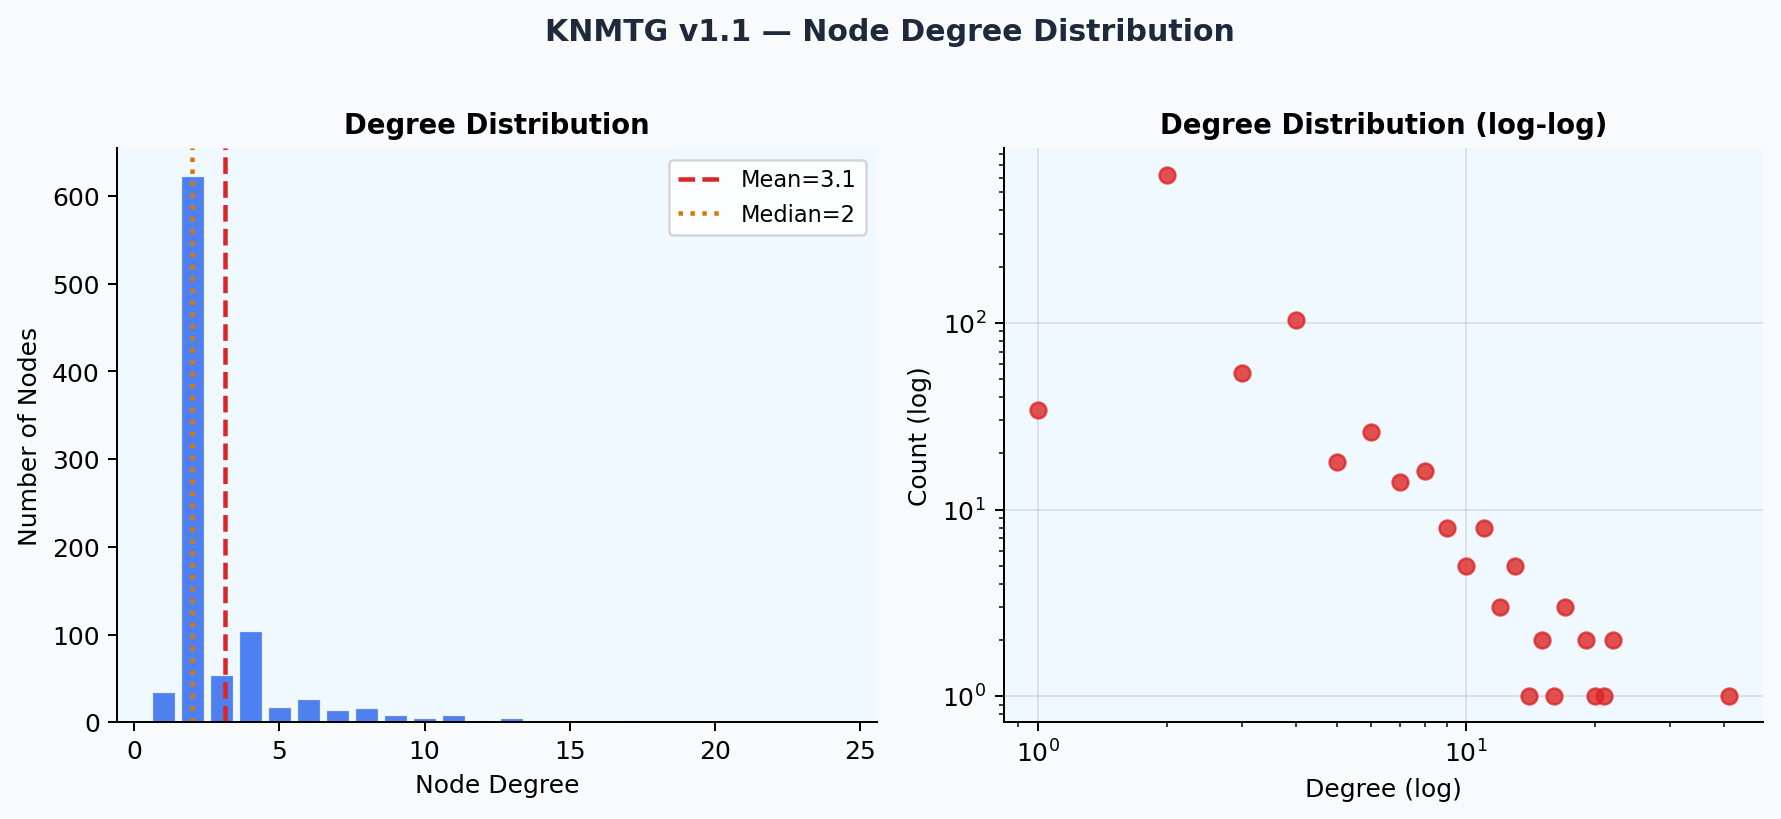
\includegraphics[width=0.7\textwidth]{fig2_degree_dist.png}
\caption{Degree distribution of KNMTG v1.1 (932 nodes).}
\label{fig:degree}
\end{figure}

\section*{S4. Midpoint Scoring Function}

Given $n$ origins and travel-time maps $d_i: V \rightarrow \mathbb{R}_{\geq 0}$,
the composite score for candidate node $v$ under strategy $s$ is:

\begin{equation}
\text{score}_s(v) = w^s_{\max} \cdot \max_i d_i(v)
                  + w^s_{\text{sum}} \cdot \sum_i d_i(v)
                  + w^s_{\sigma} \cdot \sigma\bigl(d_i(v)\bigr)
                  - w^s_{\text{pr}} \cdot \text{PageRank}(v)
\end{equation}

Table~\ref{tab:weights} lists the weight vectors for each strategy.

\begin{table}[h]
\centering
\caption{Strategy weight parameters}
\label{tab:weights}
\begin{tabular}{lrrrr}
\toprule
Strategy & $w_{\max}$ & $w_{\text{sum}}$ & $w_{\sigma}$ & $w_{\text{pr}}$ \\
\midrule
Balanced (default) & 0.5 & 0.3 & 0.2 & 50 \\
Minimize-max       & 1.0 & 0.1 & 0.1 & 20 \\
Minimize-sum       & 0.1 & 1.0 & 0.1 & 20 \\
\bottomrule
\end{tabular}
\end{table}

\section*{S5. Data Availability}

The full KNMTG v1.1 dataset (nodes, edges, routing code) is publicly
available at \url{https://github.com/yongjun-kim/knmtg} under CC-BY 4.0
(data) and MIT (code) licenses.

\end{document}
